
\documentclass[12pt,a4paper]{article}
\usepackage[latin1]{inputenc}
\usepackage{amsmath}
\usepackage{amsfonts}
\usepackage{amssymb}
\usepackage{scalefnt}
\usepackage{titlesec}
\usepackage{hyperref}

\usepackage{cite}
\usepackage{graphicx}
\usepackage{wrapfig}
\usepackage{xcolor}
\usepackage{fancyvrb}

%\usepackage{tikz}
%\usepackage{pgflibraryarrows}
%\usepackage{pgflibrarysnakes}
%\usetikzlibrary{decorations.markings}
%\usetikzlibrary{patterns,fadings}

\addtolength{\hoffset}{-4em}
\addtolength{\textwidth}{8em}
\addtolength{\voffset}{-4em}
\addtolength{\textheight}{8em}
\setlength{\parindent}{2em}
\linespread{1.1} % also in front page

\renewcommand\FancyVerbTab{\textcolor{tabcolor}{$\mid$}}

\newcommand*{\justifyheading}{\centering}
\titleformat{\section}
  {\normalfont\Huge\bfseries\justifyheading}{\thesection}{1em}{}
\titleformat{\subsection}
  {\normalfont\Large\bfseries}{\thesubsection}{1em}{}

\usepackage{listings}

\lstset{ %
language=C,                     % choose the language of the code
basicstyle=\small\ttfamily,       % the size of the fonts that are used for the code
numbers=left,                   % where to put the line-numbers
numberstyle=\small\ttfamily,      % the size of the fonts that are used for the line-numbers
stepnumber=1,                   % the step between two line-numbers. If it's 1 each line will be numbered
numbersep=5pt,                  % how far the line-numbers are from the code
backgroundcolor=\color{white},  % choose the background color. You must add \usepackage{color}
showspaces=false,               % show spaces adding particular underscores
showstringspaces=false,         % underline spaces within strings
showtabs=false,                 % show tabs within strings adding particular underscores
frame=single,                  % adds a frame around the code
tabsize=2,                    % sets default tabsize to 2 spaces
captionpos=b,                   % sets the caption-position to bottom
breaklines=true,                % sets automatic line breaking
breakatwhitespace=false,        % sets if automatic breaks should only happen at whitespace
escapeinside={\%*}{*)}          % if you want to add a comment within your code
}
\title{CD-HIT User's Guide }

\date{}
\begin{document}
\scalefont{1.1}
\maketitle
\vspace{10em}
\begin{center}

Last updated: 2012-04-25

\href{http:\slash \slash cd-hit.org}{http:\slash \slash cd-hit.org}

\href{http:\slash \slash bioinformatics.org\slash cd-hit\slash }{http:\slash \slash bioinformatics.org\slash cd-hit\slash }

Program developed by Weizhong Li's lab at UCSD \href{http:\slash \slash weizhong-lab.ucsd.edu}{http:\slash \slash weizhong-lab.ucsd.edu} \href{liwz@sdsc.edu}{liwz@sdsc.edu}

\end{center}

\clearpage
\tableofcontents
\clearpage

\clearpage
\section{Introduction }

CD-HIT was originally a protein clustering program. The main advantage of this program is its ultra-fast speed. It can be hundreds of times faster than other clustering programs, for example, BLASTCLUST. Therefore it can handle very large databases, like NR.

The 1st version of this program, CD-HI, was published and released in 2001. The 2nd version, called CD-HIT, was published in 2002 with significant improvements. Since 2004, CD-HIT has been hosted at bioinformatics.org as an open source project.

Since its release, CD-HIT has been getting more and more popular. It has a significant user base, I estimated at over several thousands users. It is used at many research and educational institutions. For example, at {\bf UniProt}, CD-HIT is used to generate the {\bf UniRef} reference data sets (\href{http:\slash \slash www.pir.uniprot.org\slash database\slash DBDescription.shtml}{http:\slash \slash www.pir.uniprot.org\slash database\slash DBDescription.shtml}). It is also used in {\bf PDB} to treat redundant sequences (\href{http:\slash \slash rutgers.rcsb.org\slash pdb\slash redundancy.html}{http:\slash \slash rutgers.rcsb.org\slash pdb\slash redundancy.html}).

In 2006, the 3rd major updates were published and released with abilities to perform various jobs like clustering a protein database, clustering a DNA/RNA database, comparing two databases (protein or DNA/RNA), generating protein families, and many others.

The CD-HIT web server was implemented in 2009, which allows users to cluster or compare sequences without using command CD-HIT. The server provides interactive interface and additional visualization tools. It also provides pre-calculated and regularly updated sequence clusters for several widely used databases.

CD-HIT-454, a special version of CD-HIT was implemented in 2010 to cluster artificial duplicated reads in pyrosequencing (454) data.

Currently, CD-HIT package has many programs: cd-hit, cd-hit-2d, cd-hit-est, cd-hit-est-2d, cd-hit-para, cd-hit-2d-para, psi-cd-hit, psi-cd-hit-2d, cd-hit-454. I also developed some utility tools, written in Perl, to help run and analyze CD-HIT jobs.

This program is still under active development; new features and new programs will be out in the future.
It can be copied under the GNU General Public License version 2 (GPLv2).

\clearpage
\section{Algorithm }

Algorithms for CD-HIT were described in three papers published in Bioinformatics.

\begin{itemize}
 \item 1. Clustering of highly homologous sequences to reduce the size of large protein databases. Weizhong Li, Lukasz Jaroszewski \& Adam Godzik. Bioinformatics (2001) 17:282-283, \href{http:\slash \slash bioinformatics.oupjournals.org\slash cgi\slash reprint\slash 17\slash 3\slash 282.pdf}{PDF}, \href{http:\slash \slash www.ncbi.nlm.nih.gov\slash entrez\slash query.fcgi?cmd=Retrieve&db=pubmed&dopt=Abstract&list_uids=11294794}{Pubmed}

\item 2. Tolerating some redundancy significantly speeds up clustering of large protein databases. Weizhong Li, Lukasz Jaroszewski \& Adam Godzik. Bioinformatics (2002) 18: 77-82, \href{http:\slash \slash bioinformatics.oupjournals.org\slash cgi\slash reprint\slash 18\slash 1\slash 77.pdf}{PDF}, \href{http:\slash \slash www.ncbi.nlm.nih.gov\slash entrez\slash query.fcgi?cmd=Retrieve&db=pubmed&dopt=Abstract&list_uids=11836214}{Pubmed}

\item 3. Cd-hit: a fast program for clustering and comparing large sets of protein or nucleotide sequences. Weizhong Li \& Adam Godzik. Bioinformatics (2006) 22:1658-1659 \href{http:\slash \slash bioinformatics.oxfordjournals.org\slash cgi\slash reprint\slash 22\slash 13\slash 1658}{PDF}, \href{http:\slash \slash www.ncbi.nlm.nih.gov\slash entrez\slash query.fcgi?db=pubmed&cmd=Retrieve&dopt=Abstract&list_uids=16731699}{Pubmed}

\end{itemize}

I suggest that you read these papers if (1) you want to understand more details about the algorithm or (2) you want know why it is so fast. If you don't have time to read these papers, the algorithms are summarized below. CD-HIT web server and CD-HIT-454 are described in these two papers:

\begin{itemize}
 \item 4. Ying Huang, Beifang Niu, Ying Gao, Limin Fu and Weizhong Li. CD-HIT Suite: a web server for clustering and comparing biological sequences. Bioinformatics, (2010). 26:680 \href{http:\slash \slash bioinformatics.oxfordjournals.org\slash cgi\slash reprint\slash btq003v1}{PDF} \href{http:\slash \slash www.ncbi.nlm.nih.gov\slash pubmed\slash 20053844}{Pubmed}

\item 5. Beifang Niu, Limin Fu, Shulei Sun and Weizhong Li, Artificial and natural duplicates in pyrosequencing reads of metagenomic data. BMC Bioinformatics, (2010) 11:187 \href{http:\slash \slash www.biomedcentral.com\slash content\slash pdf\slash 1471-2105-11-187.pdf}{PDF} \href{http:\slash \slash www.ncbi.nlm.nih.gov\slash pubmed\slash 20388221}{Pubmed}

\end{itemize}

\subsection{CD-HIT clustering algorithm }

Clustering a sequence database requires all-by-all comparisons; therefore it is very time-consuming. Many methods use BLAST to compute the all vs. all similarities. It is very difficult for these methods to cluster large databases. While CD-HIT can avoid many pairwise sequence alignments with a short word filter I developed.

In CD-HIT, I use greedy incremental clustering algorithm method. Briefly, sequences are first sorted in order of decreasing length. The longest one becomes the representative of the first cluster. Then, each remaining sequence is compared to the representatives of existing clusters. If the similarity with any representative is above a given threshold, it is grouped into that cluster. Otherwise, a new cluster is defined with that sequence as the representative.

Here is how the short word filter works. Two proteins with a certain sequence identity must have at least a specific number of identical dipeptides, tripeptides and etc. For example, for two sequences to have 85\% identity over a 100-residue window they have to have at least 70 identical dipeptides, 55 identical tripeptides, and 25 identical pentapeptides. By understanding the short word requirement, CD-HIT skips most pairwise alignments because it knows that the similarity of two sequences is below certain threshold by simple word counting. 

Another reason why CD-HIT is so fast is the use of an index table. I just use very short word with size 2~5. For instance, the total number of possible pentapeptides is only 215 (each position has 21 possibilities, 20 amino acids plus "X"), and the index table requires only 4 million entries, which just matches the RAM scale of current computers. Index table makes the counting of short word very efficiently. And a longer word is more efficient than a shorter one.

\subsection{Algorithm limitations }

A limitation of short word filter is that it can not be used below certain clustering thresholds. In a worst case scenario (figure below), when mismatches are evenly distributed along the alignment, the numbers of common short words are minimal. So theoretically, pentapeptide, tetrapeptide, tripeptide and dipeptide could only be used for thresholds above 80\%, 75\%, 66.67\% and 50\% respectively.

\begin{figure}[!h]
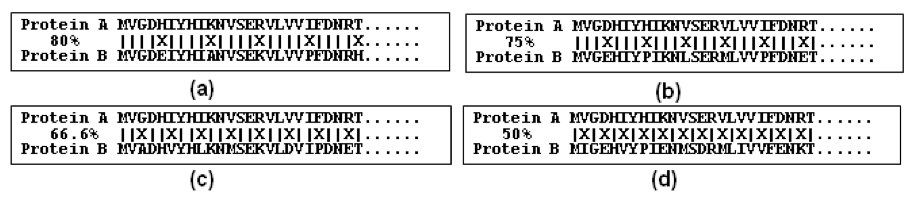
\includegraphics[width=\textwidth]{Figure1.png}

\end{figure}

Short word filtering is limited to certain clustering thresholds. Evenly distributed mismatches are shown in alignments with 80\%, 75\%, 66.67\% and 50\% sequence identities. The number of common pentapeptides in (a), tetrapeptides in (b), tripeptides in (c), and dipeptides in (d) can be zero.

However, biological sequences are not lines of random letters; proteins usually have more conserved regions and more diverse regions as the result of specific constraints of evolution. Situations such as in above figure are very rare in the real world, and the actual number of common short words is much higher than in the worst case scenarios. We did a large-scale statistical analysis on short words. We found, for example, even at 70\% identity, sequences still have statistically significant number of common pentapeptides. Current CD-HIT is based on this short word statistics. But the short word filters are still limited to certain thresholds. The reasonable limits of clustering thresholds for pentapeptide, tetrapeptide, tripeptide and dipeptide are approximately 70\%, 60\%, 50\% and 40\%, respectively.

There is another problem introduced by the greedy incremental clustering. Let say, there are two clusters: cluster \#1 has A, X and Y where A is the representative, and cluster \#2 has B and Z where B is the representative. The problem is that even if Y is more similar to B than to A, it can still in cluster \#1, simple because Y first hit A during clustering process. While this problem could be reduced by multiple-step clustering (see following sections).

\subsection{CD-HIT-2D comparing algorithm }

The above short word filtering and index table can also be used in other sequence comparison tasks, for example, comparing two data sets and reporting the matches between 2 datasets over a certain similarity threshold. This is a very common job, so I developed another program cd-hit-2d for fast comparison of two dataset.

\subsection{DNA/RNA clustering \& comparing }

The original CD-HIT was developed for protein clustering. But the short word filtering and index table implementation can also be applied to DNA/RNA. Therefore, I wrote another two new programs cd-hit-est and cd-hit-est-2d. I believe they can be very useful in handling DNA sequences.

\subsection{PSI-CD-HIT clustering }

The lowest threshold of CD-HIT is around 40\%, in many applications, people need a much lower threshold, like 25\%. I am planning to develop such application (may be called CD-HIT-LOW, I don't know yet), but for now, I use PSI-CD-HIT for this purpose.

PSI-CD-HIT is actually a Perl script I wrote, which runs similar algorithm like CD-HIT but using BLAST to calculate similarities. Below are the procedures of PSI-CD-HIT:

\begin{enumerate}
 \item  Sort sequences by decreasing length 

\item  First one is the first representative

\item  Using 1st one blast all remaining sequences, pick up its neighbors that meet the clustering threshold

\item  Repeat until done

\end{enumerate}

\subsection{CD-HIT-454 clustering }

We implemented a program called cd-hit-454 to identify duplicated 454 reads by reengineering cd-hit-est. Duplicates are either exactly identical or meet these criteria includes: (1) they start at the same position; (2) their lengths can be different, but shorter one must be fully aligned with the longer one (the seed); (3) they can only have 4\% mismatches (insertion, deletion, and substitution); and (4) only 1 base is allowed per insertion or deletion. Here, (3) and (4) can be adjusted by users. We allow mismatches in order to tolerate sequencing errors.

 

\clearpage
\section{User's Guide }

\subsection{Installation }

 

Most CD-HIT programs were written in C++. Installing CD-HIT package is very simple:

\begin{itemize}
 \item  download current CD-HIT at \href{http:\slash \slash bioinformatics.org\slash cd-hit}{http:\slash \slash bioinformatics.org\slash cd-hit}, for example cd-hit-2006-0215.tar.gz

\item  unpack the file with " tar xvf cd-hit-2006-0215.tar.gz --gunzip"

\item  change dir by "cd cd-hit-2006"

\item  compile the programs by "make"

\item  you will have all cd-hit programs compiled

\end{itemize}

\subsection{Installation of multiple threaded version }

You can take advantage of multiple-threaded function of cd-hit to speed up calculation. Please compile the programs by "make openmp=yes". OpenMP is supported in most recent Linux systems.

There are some macros defined in a cd-hi.h that control some basic parameters. I believe, in 99\% of the case, that these setting are fine. But you can change them also. I list some of them here:

\begin{lstlisting}
#define MAX_SEQ 65536
  Max length of sequences.
  
#define MAX_DIAG 133000
  This number should be the double of MAX_SEQ.

#define MAX_GAP 65536
  Max allowed gap length in dynamic programming subroutine.

#define MAX_LINE_SIZE 300000
  Max allowed length of a single line from input FASTA file.

#define MAX_FILE_NAME 1280
  Max allowed length of filename.
\end{lstlisting}

Please note that, the above values may not reflect the actual values used in the program, please refer to the source file if you want to know the exact values.

  

\subsection{CD-HIT }

CD-HIT clusters proteins into clusters that meet a user-defined similarity threshold, usually a sequence identity. Each cluster has one representative sequence. The input is a protein dataset in fasta format and the output are two files: a fasta file of representative sequences and a text file of list of clusters.

Basic command:

\begin{lstlisting}
  cd-hit -i nr -o nr100 -c 1.00 -n 5 -M 2000
  cd-hit -i db -o db90 -c 0.9 -n 5
\end{lstlisting}
where\\
\texttt{db} is the filename of input,\\
\texttt{db90} is output,\\
\texttt{0.9} means 90\% identity, is the clustering threshold\\
\texttt{5} is the size of word\\

Choose of word size:

\texttt{-n 5} for thresholds 0.7 ~ 1.0\\
\texttt{-n 4} for thresholds 0.6 ~ 0.7\\
\texttt{-n 3} for thresholds 0.5 ~ 0.6\\
\texttt{-n 2} for thresholds 0.4 ~ 0.5\\

Complete options:

{\bf The most updated options are available from the command line version of the programs. Running the programs without any argument will print out the detailed options.}

\begin{lstlisting}
-i input input filename in fasta format, required
-o output filename, required
-c sequence identity threshold, default 0.9 this is the default cd-hit's "global sequence identity" calculated as: number of identical amino acids in alignment divided by the full length of the shorter sequence
-G use global sequence identity, default 1 if set to 0, then use local sequence identity, calculated as : number of identical amino acids in alignment divided by the length of the alignment NOTE!!! don't use -G 0 unless you use alignment coverage controls see options -aL, -AL, -aS, -AS
-b band_width of alignment, default 20
-M max available memory (Mbyte), default 400
-n word_length, default 5, see user's guide for choosing it
-l length of throw_away_sequences, default 10
-t tolerance for redundance, default 2
-d length of description in .clstr file, default 20 if set to 0, it takes the fasta defline and stops at first space
-s length difference cutoff, default 0.0 if set to 0.9, the shorter sequences need to be at least 90% length of the representative of the cluster
-S length difference cutoff in amino acid, default 999999 if set to 60, the length difference between the shorter sequences and the representative of the cluster can not be bigger than 60
-aL alignment coverage for the longer sequence, default 0.0 if set to 0.9, the alignment must covers 90% of the sequence
-AL alignment coverage control for the longer sequence, default 99999999 if set to 60, and the length of the sequence is 400, then the alignment must be >= 340 (400-60) residues
-aS alignment coverage for the shorter sequence, default 0.0 if set to 0.9, the alignment must covers 90% of the sequence
-AS alignment coverage control for the shorter sequence, default 99999999 if set to 60, and the length of the sequence is 400, then the alignment must be >= 340 (400-60) residues
-uL maximum unmatched percentage for the longer sequence, default 1.0
    if set to 0.1, the unmatched region (excluding leading and tailing gaps)
    must not be more than 10% of the sequence
-uS maximum unmatched percentage for the shorter sequence, default 1.0
    if set to 0.1, the unmatched region (excluding leading and tailing gaps)
    must not be more than 10% of the sequence
-U  maximum unmatched length, default 99999999
    if set to 10, the unmatched region (excluding leading and tailing gaps)
    must not be more than 10 bases
-B 1 or 0, default 0, by default, sequences are stored in RAM if set to 1, sequence are stored on hard drive it is recommended to use -B 1 for huge databases
-p 1 or 0, default 0 if set to 1, print alignment overlap in .clstr file
-T number of threads, default 1; with 0, all CPUs will be used
-g 1 or 0, default 0 By cd-hit's default algorithm, a sequence is clustered to the first cluster that meet the threshold (fast mode). If set to 1, the program will cluster it into the most similar cluster that meet the threshold (accurate but slow mode)
\end{lstlisting}

Alignment coverage control:

See the figure below, the -aL, -AL, -aS and -AS options can be used to specify the alignment coverage on both the representative sequence and other sequences. -s and -S can control the length difference between the representative sequence and other sequences.

\begin{figure}[!h]
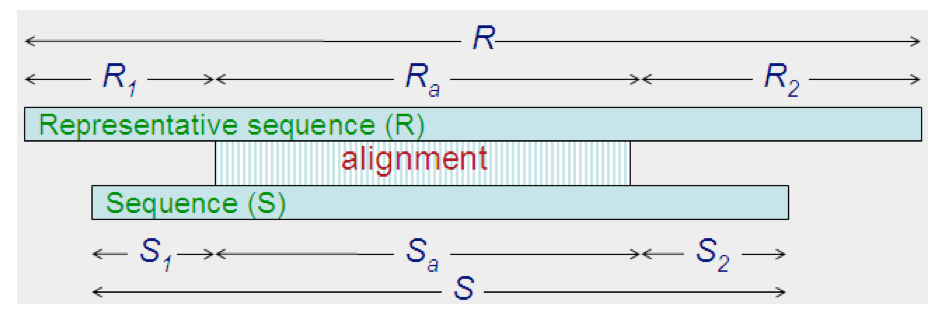
\includegraphics[width=\textwidth]{Figure2.png}

\end{figure}

\texttt{
aL = R$_a$ / R\\
AL = R - R$_a$\\
aS = S$_a$ / S\\
AS = S - S$_a$\\
s = S$_a$ / R$_a$\\
S = R / S\\
U = S$_1$ + S$_2$\\
uL = U / R\\
uS = U / S
}

Output:

The output .clstr file looks like
\begin{lstlisting}
>Cluster 0
0 2799aa, >PF04998.6|RPOC2_CHLRE/275-3073... *
>Cluster 1
0 2214aa, >PF06317.1|Q6Y625_9VIRU/1-2214... at 80%
1 2215aa, >PF06317.1|O09705_9VIRU/1-2215... at 84%
2 2217aa, >PF06317.1|Q6Y630_9VIRU/1-2217... *
3 2216aa, >PF06317.1|Q6GWS6_9VIRU/1-2216... at 84%
4 527aa, >PF06317.1|Q67E14_9VIRU/6-532... at 63%
>Cluster 2
0 2202aa, >PF06317.1|Q6UY61_9VIRU/8-2209... at 60%
1 2208aa, >PF06317.1|Q6IVU4_JUNIN/1-2208... *
2 2207aa, >PF06317.1|Q6IVU0_MACHU/1-2207... at 73%
3 2208aa, >PF06317.1|RRPO_TACV/1-2208... at 69%
\end{lstlisting}

where\\
a "$>$" starts a new cluster\\
a "*" at the end means that this sequence is the representative of this cluster\\
a "\%" is the identity between this sequence and the representative

\subsection{CD-HIT-2D }

CD-HIT-2D compares 2 protein datasets (db1, db2). It identifies the sequences in db2 that are similar to db1 at a certain threshold. The input are two protein datasets (db1, db2) in fasta format and the output are two files: a fasta file of proteins in db2 that are not similar to db1 and a text file that lists similar sequences between db1 \& db2.

Basic command:

\begin{lstlisting}
  cd-hit-2d -i db1 -i2 db2 -o db2novel -c 0.9 -n 5
\end{lstlisting}
where\\
\texttt{db1} \& \texttt{db2} are inputs,\\
\texttt{db2novel} is output,\\
\texttt{0.9} means 90\% identity, is the comparing threshold\\
\texttt{5} is the size of word

Please note that by default, I only list matches where sequences in db2 are
not longer than sequences in db1. You may use options -S2 or -s2 to overwrite
this default. You can also run command:

\begin{lstlisting}
  cd-hit-2d -i db2 -i2 db1 -o db1novel -c 0.9 -n 5  
\end{lstlisting}

Choose of word size (same as cd-hit):
\begin{lstlisting}
-n 5 for thresholds 0.7 ~ 1.0
-n 4 for thresholds 0.6 ~ 0.7
-n 3 for thresholds 0.5 ~ 0.6
-n 2 for thresholds 0.4 ~ 0.5 
\end{lstlisting}

More options:

Options, -b, -M, -l, -d, -t, -s, -S, -B, -p, -aL, -AL, -aS, -AS, -g, -G, -T
are same to CD-HIT, here are few more cd-hit-2d specific options:
\begin{lstlisting}
-i2 input filename for db2 in fasta format, required
-s2 length difference cutoff for db1, default 1.0
    by default, seqs in db1 >= seqs in db2 in a same cluster
    if set to 0.9, seqs in db1 may just >= 90% seqs in db2
-S2 length difference cutoff, default 0
    by default, seqs in db1 >= seqs in db2 in a same cluster
    if set to 60, seqs in db2 may 60aa longer than seqs in db1
\end{lstlisting}

\subsection{CD-HIT-EST }

CD-HIT-EST clusters a nucleotide dataset into clusters that meet a
user-defined similarity threshold, usually a sequence identity. The input is
a DNA/RNA dataset in fasta format and the output are two files: a fasta file
of representative sequences and a text file of list of clusters. 
Since eukaryotic genes usually have long introns, which cause long gaps, it is
difficult to make full-length alignments for these genes. So, CD-HIT-EST is
good for non-intron containing sequences like EST.  

Basic command:

\begin{lstlisting}
  cd-hit-est -i est_human -o est_human95 -c 0.95 -n 8  
\end{lstlisting}

Choose of word size:
\begin{lstlisting}
-n 8,9,10 for thresholds 0.90 ~ 1.0
-n 7      for thresholds 0.88 ~ 0.9
-n 6      for thresholds 0.85 ~ 0.88
-n 5      for thresholds 0.80 ~ 0.85
-n 4      for thresholds 0.75 ~ 0.8 
\end{lstlisting}

More options:

Options, -b, -M, -l, -d, -t, -s, -S, -B, -p, -aL, -AL, -aS, -AS, -g, -G, -T
are same to CD-HIT, here are few more cd-hit-est specific options:
\begin{lstlisting}
-r 1 or 0, default 0, if set to 1, comparing both strand (++, +-)
\end{lstlisting}

\subsection{CD-HIT-EST-2D }

CD-HIT-EST-2D compares 2 nucleotide datasets (db1, db2). It identifies the
sequences in db2 that are similar to db1 at a certain threshold. The input are
two DNA/RNA datasets (db1, db2) in fasta format and the output are two files:
a fasta file of sequences in db2 that are not similar to db1 and a text file
that lists similar sequences between db1 \& db2.  
For same reason as CD-HIT-EST, CD-HIT-EST-2D is good for non-intron containing
sequences like EST.  

Basic command:

\begin{lstlisting}
  cd-hit-est-2d -i mrna_human -i2 est_human -o est_human_novel -c 0.95 -n 8  
\end{lstlisting}

Choose of word size (same as CD-HIT-EST):
\begin{lstlisting}
-n 8,9,10 for thresholds 0.90 ~ 1.0
-n 7      for thresholds 0.88 ~ 0.9
-n 6      for thresholds 0.85 ~ 0.88
-n 5      for thresholds 0.80 ~ 0.85
-n 4      for thresholds 0.75 ~ 0.8 
\end{lstlisting}

More options:

Options, -b, -M, -l, -d, -t, -s, -S, -s2, -S2, -B, -p, -aL, -AL, -aS, -AS, -g,
-G, -T are same to CD-HIT-2d, here are few more cd-hit-est-2d specific
options:
\begin{lstlisting}
-r 1 or 0, default 0, if set to 1, comparing both strand (++, +-)
\end{lstlisting}

\subsection{Multi-threaded programs }

Multi-threaded cd-hit programs were implemented with OpenMP. Option "-T
n" will enable cd-hit to run in parallel in a single multi-core computer.
The default value of n is 1 (single thread). "-T 0" will use all the
cores in that computer. We have run cd-hit on 4-core, 8-core to 32-core
computers and have observed a great speedup.

\subsection{CD-HIT-PARA }

CD-HIT-PARA is a script that runs cd-hit, cd-hit-est in a parallel mode. It
splits the input database; runs cd-hit or cd-hit-est in parallel on a computer
cluster; and finally merges the outputs into a single file.  You can run it as
you run cd-hit or cd-hit-est. The input is a protein or DNA/RNA dataset in
fasta format and the output are two files: a fasta file of representative
sequences and a text file of list of clusters. 

There are two ways to run jobs on a cluster: by ssh to a remote computer and
by queuing system (PBS and SGE are implemented). In any case, you should have
a shared file system, the path to your working directory must be same on all
the remote computers. 

This script can also be used if you are clustering a very large database and
your computer doesn't have enough RAM. In that case, all the divided jobs
will still run on a single computer. 

Implementation (see figure below)

\begin{enumerate}
 \item  divide input db into many small dbs in decreasing length

\item  clusters the 1st db by cd-hit

\item  run cd-hit-2d for other dbs against 1st db

\item  repeat cd-hit and cd-hit-2d runs till done

\item  Combine the results

\end{enumerate}

\begin{figure}[!h]
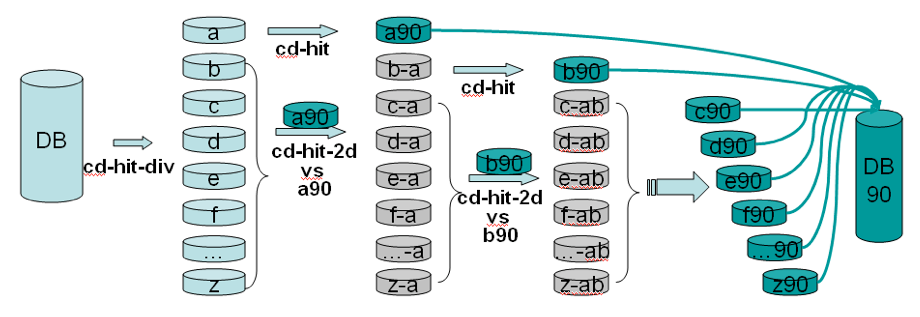
\includegraphics[width=\textwidth]{Figure3.png}

\end{figure}

Basic command:

\begin{lstlisting}
  cd-hit-para.pl -i nr90 -o nr60 -c 0.6 -n 4 --B hosts --S 64
\end{lstlisting}

  
where\\
\texttt{--B} hosts is a file with available hostnames\\
\texttt{--S} 64 is the number to split input db into, this number should be several times the number of hosts 

More options:
\begin{lstlisting}
--P program, "cd-hit" or "cd-hit-est", default "cd-hit"
--B filename of list of hosts,
    requred unless -Q or -L option is supplied
--L number of cpus on local computer, default 0
    when you are not running it over a cluster, you can use
    this option to divide a big clustering jobs into small
    pieces, I suggest you just use "--L 1" unless you have
    enough RAM for each cpu
--S Number of segments to split input DB into, default 64
--Q number of jobs to submit to queue queuing system, default 0
    by default, the program use ssh mode to submit remote jobs
--T type of queuing system, "PBS", "SGE" are supported, default PBS
--R restart file, used after a crash of run
\end{lstlisting}

\subsection{CD-HIT-2D-PARA }

CD-HIT-2D-PARA is a script that runs cd-hit-2d, cd-hit-est-2d in a parallel
mode. It splits the input databases; runs cd-hit-2d or cd-hit-est-2d in
parallel on a computer cluster; and finally merges the outputs into a single
file.  You can run it as you run cd-hit-2d or cd-hit-est-2d. The input is a
protein or DNA/RAN dataset in fasta format and the output are two files: a
fasta file of representative sequences and a text file of list of clusters. 

Basic command:

\begin{lstlisting}
  cd-hit-para.pl -i nr -i2 swissprot -o swissprot_vs_nr -c 0.6 -n 4 --Q 20 -T "SGE" --S 2 --S2 20
\end{lstlisting}

  
where  
\begin{lstlisting}
    --P  program, "cd-hit-2d" or "cd-hit-est-2d",
         default "cd-hit-2d"
    --B  filename of list of hosts,
         requred unless -Q or -L option is supplied
    --L  number of cpus on local computer, default 0
         when you are not running it over a cluster, you can use
         this option to divide a big clustering jobs into small
         pieces, I suggest you just use "--L 1" unless you have
         enough RAM for each cpu
    --S  Number of segments to split 1st db into, default 2
    --S2 Number of segments to split 2nd db into, default 8
    --Q  number of jobs to submit to queue queuing system, default 0
         by default, the program use ssh mode to submit remote jobs
    --T  type of queuing system, "PBS", "SGE" are supported, default PBS
    --R  restart file, used after a crash of run
     -h  print this help
\end{lstlisting}

\subsection{PSI-CD-HIT clustering }

PSI-CD-HIT clusters proteins into clusters that meet a user-defined similarity
threshold, which can be identity or expect value. Each cluster has one
representative sequence. The input is a protein dataset in fasta format and
the outputs are two files: a fasta file of representative sequences and a text
file of list of clusters 

Basic command:

\begin{lstlisting}
  psi-cd-hit.pl -i nr60 -o nr30 -c 0.3
  psi-cd-hit.pl -i nr60 -o nr30 -c 0.3 -b hosts 
\end{lstlisting}

\begin{lstlisting}
 
More options:
\end{lstlisting}

Options, -l, -d, -s, -S are same to CD-HIT, here are few more psi-cd-hit
specific options:
\begin{lstlisting}
-ce clustering threshold (blast expect), default -1, by default it doesn't use
    expect threshold, but with positive value, the program cluster sequences if
    similarities meet either identity threshold or expect value threshold
-L  coverage of shorter sequence (aligned / full), default 0
-M  coverage of longer sequence (aligned / full), default 0
-R  (1/0) use psi-blast profile? default 0, perform psi-blast / pdb-blast type
    search
-G  (1/0) use global identity? default 1, sequence identity calculated as
    total identical residues of local alignments / length of shorter sequence
-be blast expect cutoff, default 0.000001
-b  filename of list of hosts, to run this program in parallel with ssh calls
\end{lstlisting}

\subsection{Incremental clustering }

It is easy to make incremental update with cd-hit /cd-hit-2d. For example:

\begin{lstlisting}
  nr is the nr database of last month
  month is the new sequences of nr of this month
\end{lstlisting}

In last month, you ran:

\begin{lstlisting}
  cd-hit -i nr -o nr90 -c 0.9 -n 5
\end{lstlisting}

This month, you can run incremental clustering

\begin{lstlisting}
  cd-hit-2d -i nr90 -i2 month -o month-new -c 0.9 -n 5
  cd-hit -i month-new -o month90 -c 0.9 -n 5
  cat month90 >> nr90
  clstr_merge.pl nr90.clstr month-new.clstr > temp.clstr
  cat temp.clstr month90.clstr > this_month_nr90.clstr 
\end{lstlisting}

This approach is much faster than runing from scratch. It also preserves
stable cluster structure. 

\subsection{Hierarchically clustering }

With multiple-step, iterated runs of CD-HIT, you perform a clustering in a
neighbor-joining method, which generates a hierarchical structure.  

    

\begin{figure}[!h]
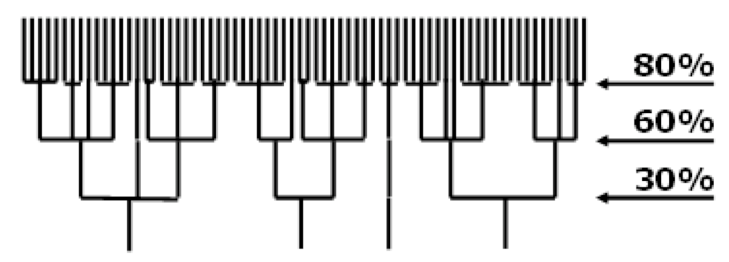
\includegraphics[width=\textwidth]{Figure4.png}

\end{figure}

Commands:

\begin{lstlisting}
  cd-hit -i nr -o nr80 -c 0.8 -n 5
  cd-hit -i nr80 -o nr60 -c 0.6 -n 4
  psi-cd-hit.pl -i nr60 -o nr30 -c 0.3
\end{lstlisting}

This way is faster than one-step run from nr directly to nr30. It can also
helps correct errors by one-step clustering (see last paragraph in algorithm
limitation section).  

\clearpage
\section{CD-HIT tools }

\subsection{cd-hit-div, cd-hit-div.pl }

Both the executable binary program cd-hit-div and the perl script divide a FASTA file into pieces. The difference is that cd-hit-div sorts the sequences before dividing them while the perl script does not.

Commands:

\begin{lstlisting}
  cd-hit-div -i input -o output -div n
  cd-hit-div.pl input output n
\end{lstlisting}

where "n" is the number of output files. The output files will be named as output-0, output-1 etc.

\subsection{plot\_len.pl }

This is a script to print out distributions of clusters \& sequences.  

Commands:

\begin{lstlisting}
  plot_len.pl input.clstr \
  1,2-4,5-9,10-19,20-49,50-99,100-299,500-99999 \
  10-59,60-149,150-499,500-1999,2000-999999
\end{lstlisting}

where

\begin{lstlisting}
  2nd line are sizes of cluster
  3rd line are lengths of sequences 
\end{lstlisting}

It will print distribution of clusters and sequences :

\begin{lstlisting}
Size    # seq   #clstr  10-59   60-149  150-499 500-1999 2000-up
1       266312  266312  36066   103737  103285  22727   497
2-4     208667  81131   1229    14680   44607   20006   609
5-9     156558  24198   118     2148    12026   9388    518
10-19   155387  11681   30      596     5024    5462    569
20-49   176815  6007    6       139     2212    3135    515
50-99   106955  1568    0       24      410     955     179
100-499 154209  896     0       3       124     597     172
500-up  43193   40      0       0       1       14      25
Total   1268096 391833  37449   121327  167689  62284   3084
\end{lstlisting}

\subsection{clstr\_sort\_by.pl }

This script sort clusters in .clstr file by length, size

Commands:

\begin{lstlisting}
  Clstr_sort_by.pl input.clstr no > input_sort.clstr
\end{lstlisting}
Where, "no" means by size of the cluster

\subsection{clstr\_sort\_prot\_by.pl }

This script sort sequences within clusters in .clstr file by length, name, etc.

Commands:

\begin{lstlisting}
  Clstr_sort_prot_by.pl input.clstr id > input_sort.clstr
\end{lstlisting}
Where, "no" means by id of sequences

\subsection{clstr\_merge.pl }

It merges two or more .clstr files. The cluster orders need to be identical.

Commands:

\begin{lstlisting}
  cd-hit-2d -i db1 -i2 db2 -o db2new -c 0.9 -n 5
  cd-hit-2d -i db1 -i2 db3 -o db3new -c 0.9 -n 5
  clstr_merge.pl db2new.clstr db3new.clstr > db23new.clstr
\end{lstlisting}

\subsection{clstr\_merge\_noorder.pl }

It merges two or more .clstr files. The cluster orders do not have to be identical.

Commands:

\begin{lstlisting}
  cd-hit-2d -i db1 -i2 db2 -o db2new -c 0.9 -n 5
  cd-hit-2d -i db1 -i2 db3 -o db3new -c 0.9 -n 5
  clstr_merge_noorder.pl db2new.clstr db3new.clstr > db23new.clstr
\end{lstlisting}

\subsection{clstr\_ renumber.pl }

It renumbers clusters and sequences within clusters in .clstr file after merge
or other operations 

Commands:

\begin{lstlisting}
  Clstr_renumber.pl input.clstr > input_ren.clstr
\end{lstlisting}

\subsection{clstr\_rev.pl }

It combines a .clstr file with its parent .clstr file 

Commands:

\begin{lstlisting}
  cd-hit -i nr -o nr90 -c 0.9 -n 5
  cd-hit -i nr90 -o nr60 -c 0.6 -n 4
  clstr_rev.pl nr90.clstr nr60.clstr > nr60_from90.clstr
  psi-cd-hit -i nr60 -o nr30 -c 0.3
  clstr_rev.pl nr60_from90.clstr nr30.clstr > nr30_from90.clstr 
\end{lstlisting}

\subsection{make\_multi\_seq.pl }

This script reads the .clstr file, it generates a separate fasta file for each cluster over certain size and saves it in designated subdirectory. To run this script correctly, "-d 0" option should be used in the cd-hit run and it is better to use "-g 1" in the cd-hit run to get accurate clustering results. For example,

Commands:

\begin{lstlisting}
  cd-hit -i db -o dbout -c 0.6 -n 4 -d 0 -g 1
  make_multi_seq.pl seq_db dbout.clstr multi-seq 20
\end{lstlisting}

will generate fasta files in "multi-seq" directory for clusters with more than 20 member sequences. Files will be named as "clusterN" where "N" is serial number of a cluster.

\subsection{clstr2xml.pl }

This script converts a cluster file or combines multiple cluster files from a hierarchical cd-hit run to xml format. The output is sorted by sequence length (default) or cluster size. The input cluster files must be in the order of being generated, that is, the cluster file with higher identity cutoff comes first.

Command:

\begin{lstlisting}
  clstr2xml.pl [-len|-size] input1.clstr [input2.clstr input3.clstr ...]
\end{lstlisting}

\clearpage
\section{CD-HIT Web Server }

The CD-HIT web server is available from \href{http:\slash \slash cd-hit.org}{http:\slash \slash cd-hit.org}. All basic functions
of CD-HIT are provided through tab-based interfaces in our web server. For
CD-HIT and CD-HIT-EST, users can upload a FASTA file, select a desired
sequence identity level and other parameters. CD-HIT-2D (CD-HIT-EST-2D) can
compare two databases uploaded by users. H-CD-HIT and H-CD-HIT-EST in our
server performs hierarchical clustering up to 3 steps. 

The CD-HIT-454 web server is also available from \href{http:\slash \slash cd-hit.org}{http:\slash \slash cd-hit.org}. 

\clearpage
\section{References }

If you find cd-hit helpful to your research and study, please kindly cite the
relevant references from the list below. 

\begin{enumerate}
 \item  Clustering of highly homologous sequences to reduce the size of large protein databases. Weizhong Li, Lukasz Jaroszewski \& Adam Godzik. Bioinformatics (2001) 17:282-283, \href{http:\slash \slash bioinformatics.oupjournals.org\slash cgi\slash reprint\slash 17\slash 3\slash 282.pdf}{PDF}, \href{http:\slash \slash www.ncbi.nlm.nih.gov\slash entrez\slash query.fcgi?cmd=Retrieve&db=pubmed&dopt=Abstract&list_uids=11294794}{Pubmed}

\item  Tolerating some redundancy significantly speeds up clustering of large protein databases. Weizhong Li, Lukasz Jaroszewski \& Adam Godzik. Bioinformatics (2002) 18: 77-82, \href{http:\slash \slash bioinformatics.oupjournals.org\slash cgi\slash reprint\slash 18\slash 1\slash 77.pdf}{PDF}, \href{http:\slash \slash www.ncbi.nlm.nih.gov\slash entrez\slash query.fcgi?cmd=Retrieve&db=pubmed&dopt=Abstract&list_uids=11836214}{Pubmed}

\item  Cd-hit: a fast program for clustering and comparing large sets of protein or nucleotide sequences. Weizhong Li \& Adam Godzik. . Bioinformatics (2006) 22:1658-1659, \href{http:\slash \slash bioinformatics.oxfordjournals.org\slash cgi\slash reprint\slash 22\slash 13\slash 1658}{PDF}, \href{http:\slash \slash www.ncbi.nlm.nih.gov\slash entrez\slash query.fcgi?db=pubmed&cmd=Retrieve&dopt=Abstract&list_uids=16731699}{Pubmed}

\item  Ying Huang, Beifang Niu, Ying Gao, Limin Fu and Weizhong Li. CD-HIT Suite: a web server for clustering and comparing biological sequences. Bioinformatics, (2010). 26:680 \href{http:\slash \slash bioinformatics.oxfordjournals.org\slash cgi\slash reprint\slash btq003v1}{PDF} \href{http:\slash \slash www.ncbi.nlm.nih.gov\slash pubmed\slash 20053844}{Pubmed}

\item  Beifang Niu, Limin Fu, Shulei Sun and Weizhong Li, Artificial and natural duplicates in pyrosequencing reads of metagenomic data. BMC Bioinformatics, (2010), 11:187 \href{http:\slash \slash www.biomedcentral.com\slash content\slash pdf\slash 1471-2105-11-187.pdf}{PDF} \href{http:\slash \slash www.ncbi.nlm.nih.gov\slash pubmed\slash 20388221}{Pubmed}

\end{enumerate}

\end{document}